\documentclass[tikz,border=6pt]{standalone}
\usepackage[T1]{fontenc}
\usepackage[utf8]{inputenc}
\usepackage{pgfplots}
\usepgfplotslibrary{groupplots}
\usetikzlibrary{calc}
\pgfplotsset{compat=1.18}
\begin{document}
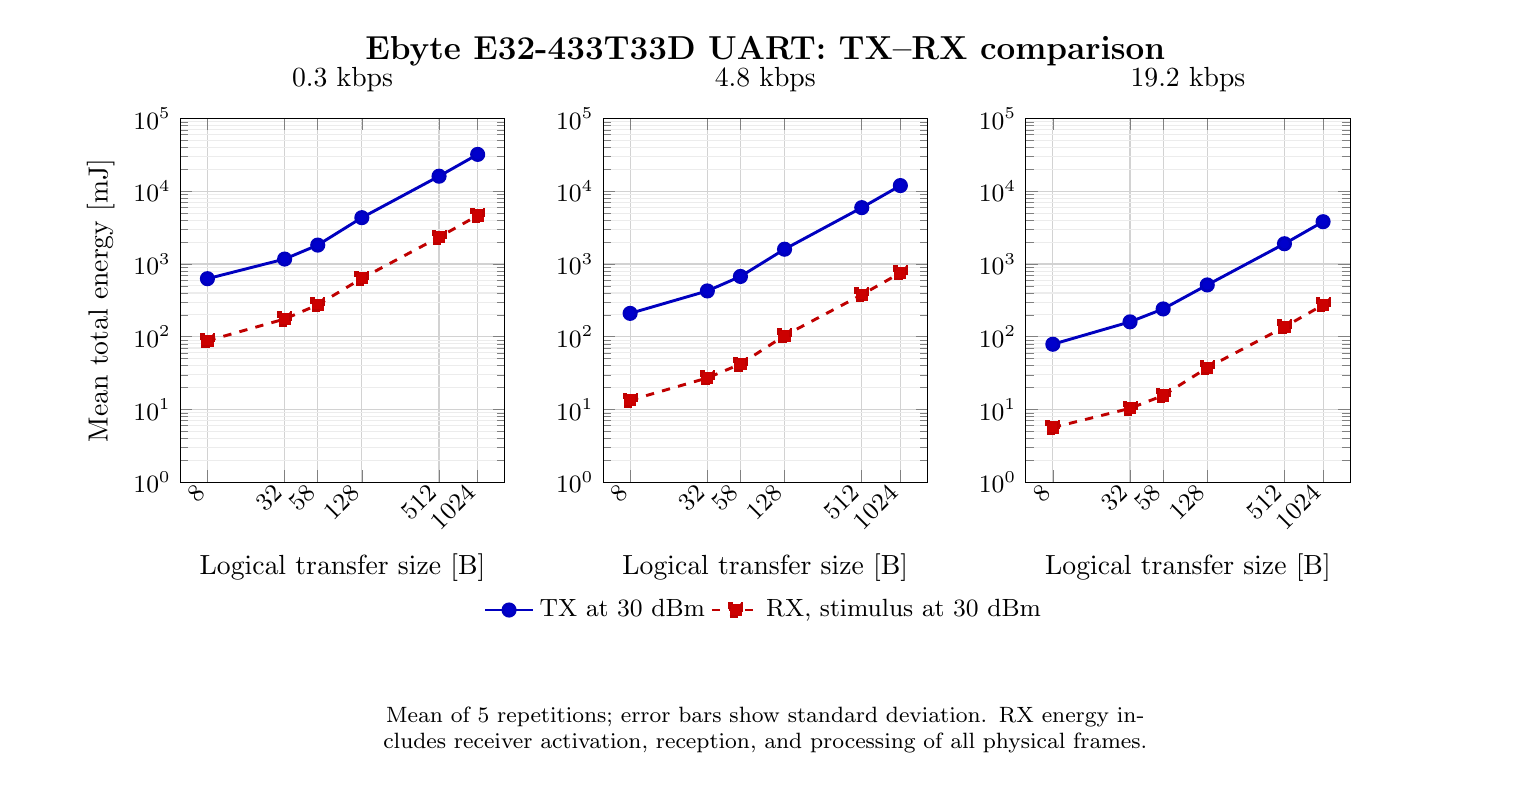
\begin{tikzpicture}
\begin{groupplot}[/pgf/number format/use comma,
  group style={group size=3 by 1, horizontal sep=1.25cm},
  width=5.7cm, height=6.2cm,
  xmode=log, log basis x={2}, ymode=log, log basis y={10},
  ymin=1, ymax=100000,
  xtick={8,32,58,128,512,1024}, xticklabels={8,32,58,128,512,1024},
  x tick label style={rotate=45, anchor=east, font=\small},
  y tick label style={font=\small},
  grid=both, minor grid style={gray!15}, major grid style={gray!35},
  xlabel={Logical transfer size [B]},
  every axis plot/.append style={line width=1.05pt},
  error bars/error bar style={line width=0.35pt},
  legend style={font=\small, draw=none, fill=none, at={(0.5,-0.29)},
    anchor=north, legend columns=-1},
]
\nextgroupplot[title={0.3 kbps}, ylabel={Mean total energy [mJ]}]
\addplot+[color=blue!75!black, solid, mark=*, mark size=2.2pt,
  error bars/.cd, y dir=both, y explicit,
] coordinates {
  (8,628.737694) +- (0,0.670410327)
  (32,1170.90249) +- (0,4.93153189)
  (58,1821.94434) +- (0,4.66547637)
  (128,4342.08191) +- (0,6.72239411)
  (512,16129.1662) +- (0,27.8234413)
  (1024,32183.0747) +- (0,185.95773)
};
\addplot+[color=red!75!black, dashed, mark=square*, mark size=2.2pt,
  error bars/.cd, y dir=both, y explicit,
] coordinates {
  (8,88.0322374) +- (0,0.495543461)
  (32,175.475611) +- (0,0.785647258)
  (58,275.019703) +- (0,1.31902768)
  (128,635.343251) +- (0,5.50151128)
  (512,2342.17156) +- (0,17.7586948)
  (1024,4641.61453) +- (0,20.1221706)
};
\nextgroupplot[title={4.8 kbps}]
\addplot+[color=blue!75!black, solid, mark=*, mark size=2.2pt,
  error bars/.cd, y dir=both, y explicit,
] coordinates {
  (8,209.670438) +- (0,0.266902432)
  (32,426.624127) +- (0,0.31013768)
  (58,675.06228) +- (0,1.21489628)
  (128,1599.47136) +- (0,3.51202573)
  (512,5961.70172) +- (0,18.7380437)
  (1024,11984.9281) +- (0,58.4610298)
};
\addlegendentry{TX at 30 dBm}
\addplot+[color=red!75!black, dashed, mark=square*, mark size=2.2pt,
  error bars/.cd, y dir=both, y explicit,
] coordinates {
  (8,13.4031066) +- (0,0.143771886)
  (32,27.1617267) +- (0,0.3543261)
  (58,42.0649902) +- (0,0.435875635)
  (128,103.723793) +- (0,0.679872919)
  (512,378.477096) +- (0,0.532168974)
  (1024,755.250477) +- (0,1.26155149)
};
\addlegendentry{RX, stimulus at 30 dBm}
\nextgroupplot[title={19.2 kbps}]
\addplot+[color=blue!75!black, solid, mark=*, mark size=2.2pt,
  error bars/.cd, y dir=both, y explicit,
] coordinates {
  (8,78.9158574) +- (0,0.0704566494)
  (32,160.354122) +- (0,0.138938939)
  (58,241.271356) +- (0,0.978260746)
  (128,515.970135) +- (0,18.4256201)
  (512,1902.11605) +- (0,24.9884352)
  (1024,3820.30682) +- (0,31.647345)
};
\addplot+[color=red!75!black, dashed, mark=square*, mark size=2.2pt,
  error bars/.cd, y dir=both, y explicit,
] coordinates {
  (8,5.64416829) +- (0,0.1869503)
  (32,10.3665802) +- (0,0.101194283)
  (58,15.5744903) +- (0,0.13156076)
  (128,37.4751016) +- (0,1.33177183)
  (512,136.488193) +- (0,2.82973147)
  (1024,274.38187) +- (0,3.03357011)
};
\end{groupplot}
\node[font=\bfseries\large] at ($(group c2r1.north)+(0,0.85cm)$)
  {Ebyte E32-433T33D UART: TX--RX comparison};
\node[font=\footnotesize, align=center, text width=18.5cm]
  at ($(group c2r1.south)+(0,-3.15cm)$)
  {Mean of 5 repetitions; error bars show standard deviation. RX energy includes receiver activation, reception, and processing of all physical frames.};
\end{tikzpicture}
\end{document}
